%\documentclass[twocolumn, trackchanges]{aastex6}
\documentclass[twocolumn]{aastex6}


\bibliographystyle{aasjournal}
\usepackage{graphicx}
\usepackage[suffix=]{epstopdf}
\usepackage{natbib}
\usepackage{amsmath}
\usepackage{url}
\usepackage{xspace}



%    Make Scientific Notation
\providecommand{\e}[1]{\ensuremath{\times 10^{#1}}}

% make the word Kepler italicized, deal w/ floating space afterwards
\newcommand{\Kepler}{\textsl{Kepler}\xspace}

\begin{document}

%%%%%%%%%%%%%%%%%%%%%%
\title{The GALEX View of ``Boyajian's Star''}

\shorttitle{GALEX View of ``Boyajian's Star''}
\shortauthors{Davenport et al.}

\author{
	James R. A. Davenport\altaffilmark{1,2}
	Riley W. Clarke\altaffilmark{1}
	Zachery Laycock\altaffilmark{1}\\
	Kevin R. Covey\altaffilmark{1}
	Scott W. Flemming\altaffilmark{3}
	Tabetha S. Boyajian\altaffilmark{4}
	Benjamin T. Montet\altaffilmark{5}\\
	Bernie Shiao\altaffilmark{3}
	Chase C. Million\altaffilmark{6}
	David J. Wilson\altaffilmark{7}
	Manuel Olmedo\altaffilmark{8}
	Eric E. Mamajek\altaffilmark{9}
	}

\altaffiltext{1}{Department of Physics \& Astronomy, Western Washington University, 516 High St., Bellingham, WA 98225, USA}
\altaffiltext{2}{NSF Astronomy and Astrophysics Postdoctoral Fellow}
 

 

%%%%%%%%%%%%%%%%%%%%%%%%%%%%%%
\begin{abstract}
The enigmatic star KIC 8462852, also known as ``Boyajian's Star'',  has puzzled for both its short (days) length dimming events, and a years-long secular dimming observed by the \Kepler mission.
GALEX provides both short timescale sampling from the photon-counting data, and longer baseline data from multiple campaigns that imaged this field/ also providing a wide wavelength baseline to compare with the optical \Kepler data, and provide important constraint for models of this system.
here we investigate both the short and long timescale data. from 4 GALEX visits totaling 1600 seconds of exposure time in 2011, spread over 70 days, we find no coherent NUV variability in the system on 10--100 sec timescales during these time windows. Comparing the integrated flux from these 2011 visits to the 2012 NUV flux published in the GALEX-CAUSE Kepler survey, we find a 3\% decrease in brightness of KIC 8462852. This decrease is the first  validation of the secular fading reported by \citet{montet2016} not in optical wavelengths. The similar amplitudes between the NUV and optical data rule out typical interstellar dust as the cause of this fading.
\end{abstract}



%%%%%%%%%%%%%%%%%%%%%%%%%%%%%%
\section{Introduction}
KIC 8462852, also known as ``Boyajian's Star'', is an unusual F3 dwarf in the \Kepler field that has exhibited unexplained optical variability on a variety of timescales. The initial discovery was of several dramatic, short timescale (days) dimming events with amplitudes up to 20\% in the \Kepler 30-min cadence data \citep{boyajian2015}. Though the \Kepler mission \citep{borucki2010} obtained data at a 30-min cadence for $\sim$4 years on this star, no definitive pattern or cycle was found, nor has any single explanation for this variability been accepted by the community \citep{wright2016b}.

Analysis of archival optical photographic plates has found that KIC 8462852 may have additionally faded nearly 16\% over the past century \citep{schaefer2016}. Such a precise measurement for a single star is difficult, and the result has been debated \citep{hippke2016}. However, using the 53 ``Full Frame Images'' (FFIs) spread over the 4-year \Kepler mission, \citet{montet2016} were able to trace the brightness of KIC 8462852 using an independent flux calibration. The resulting flux-calibrated FFI light curve showed definitively that KIC 8462852 faded by more than 3\% over 4 years. %This long timescale variability has recently been confirmed with an analysis of archival ground-based photometry (Simon et al. 2017 in prep)

The short (days) and long (years) timescale variability discovered for KIC 8462852 has presented a unique set of observational constraints on any single model used to describe the system. For example, if variable dust extinction is responsible for both temporal features, then it must have a wildly variable density distribution on small spatial scales, and a small density gradient over large spatial scales. Searches for an infrared flux excess consistent with a foreground or circumstellar dust shell have to date found no strong detection \citep{marengo2015}.


Since optical variability alone has not produced a single explanation for KIC 8462852, multi-wavelength studies are needed to constrain nature of the long timescale fading and short timescale dimming. Follow-up multi-band photometric and spectroscopic campaigns are underway\footnote{\url{http://www.wherestheflux.com}}, which will provide an improved understanding of any future ``dips''. However, to date no contemporaneous, multi-wavelength  measurement of the mysterious variability for KIC 8462852 has been available.


Archival photometry at ultraviolet wavelengths from the GALEX mission \citep{galex} is now available, and provides an important new dataset for understanding KIC 8462852. This data includes NUV monitoring over a range of time baselines, from seconds to more than a year. Time-tagged photon data has recently been made available for GALEX \citep{million2016}, including a Python toolkit to search for and interact with this high cadence data product called {\tt gPhoton} \citep{gphoton}. This allows us to resample all available GALEX survey data into any desired cadence. In the case of KIC 8462852, GALEX had $\sim$1600 seconds of data available from four separate visits spread across a $\sim$70 day baseline in 2011. In \S\ref{sec:short} we analyze this NUV data with {\tt gPhoton} sampled at a 10 second cadence, and over the whole 70 day period.




The \Kepler field was revisited by GALEX during a special campaign, dubbed the GALEX-CAUSE Kepler (hereafter GCK) survey. This survey occurred in 2012, and overlapped a portion of the Quarter 14 operations of the original \Kepler mission. Using a ``scan'' observing mode that differed from the standard GALEX survey, the GCK catalog had 1413.8 seconds of data available for KIC 8462852, which was combined into a single stacked exposure of this region \citep{olmedo2015}. Unfortunately, since the observing mode differed from the standard GALEX survey, this GCK data is not available for analysis with {\tt gPhoton} presently. In \S\ref{sec:long} we explore the long timescale evolution of KIC 8462852 between the 2011 and 2012 visits, and compare directly to the observed fading by \citet{montet2016}.

In \S\ref{sec:dust} we discuss possible interpretations for the nature of KIC 8462852 that the combined \Kepler and GALEX observations provide, including an estimate of the dust extinction properties necessary to reproduce the long timescale NUV observations. Finally in \S\ref{sec:summary} we summarize this work, and discuss the potential utility of GALEX in the study of other rare and unusual variable \Kepler objects.


%%%%%
\begin{figure}[!t]
\centering
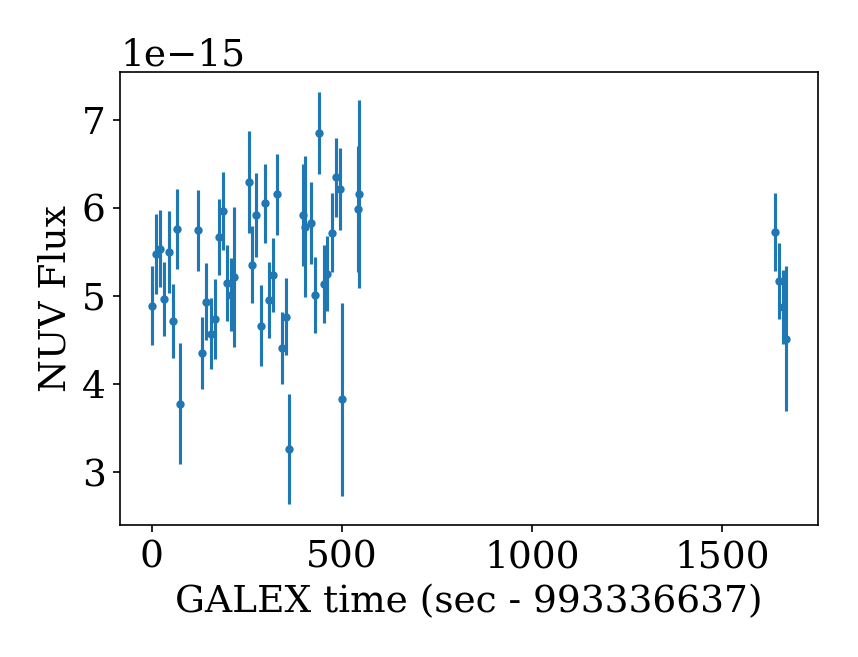
\includegraphics[width=2.7in]{KIC8462852_0_lc}
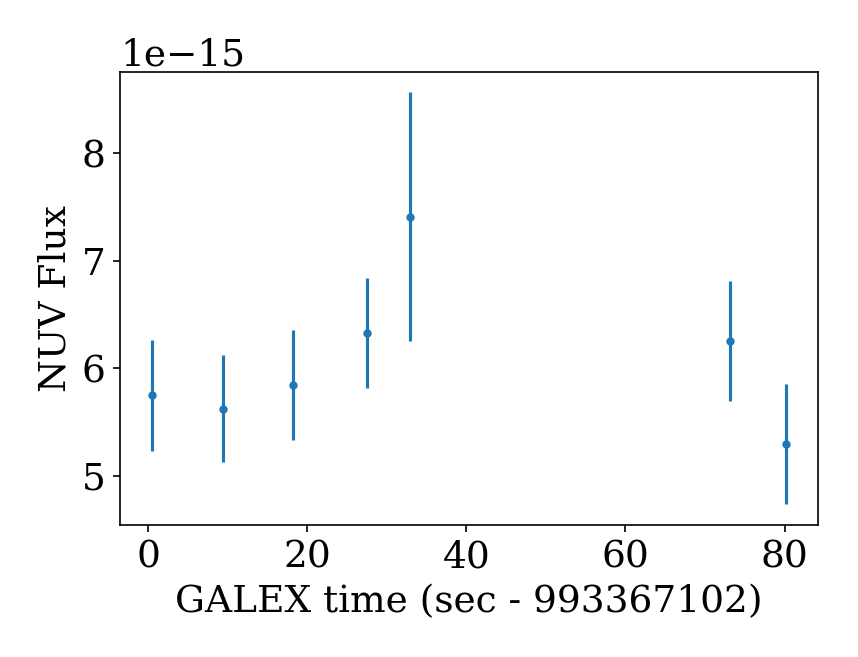
\includegraphics[width=2.7in]{KIC8462852_1_lc}
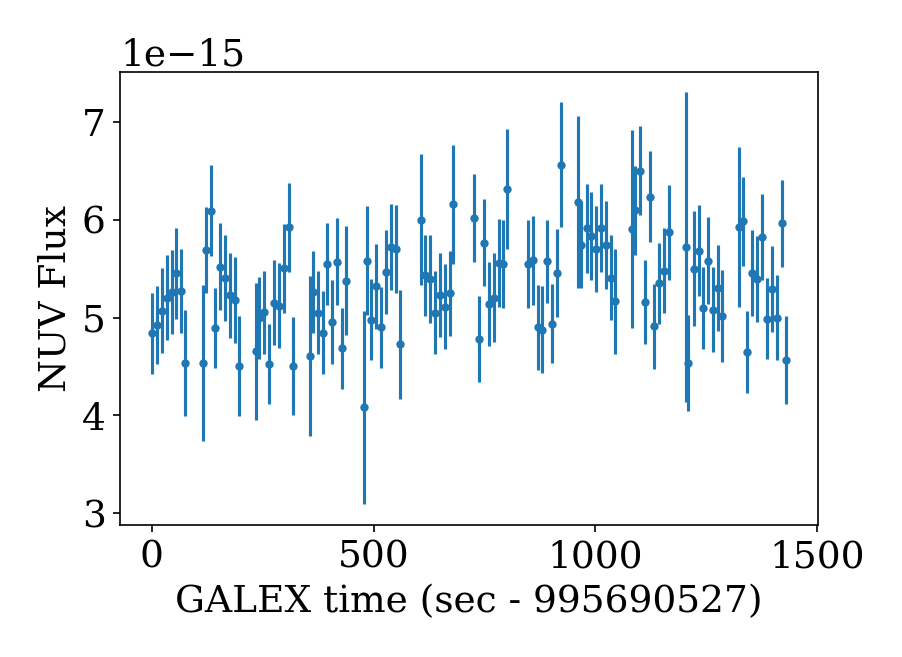
\includegraphics[width=2.7in]{KIC8462852_2_lc}
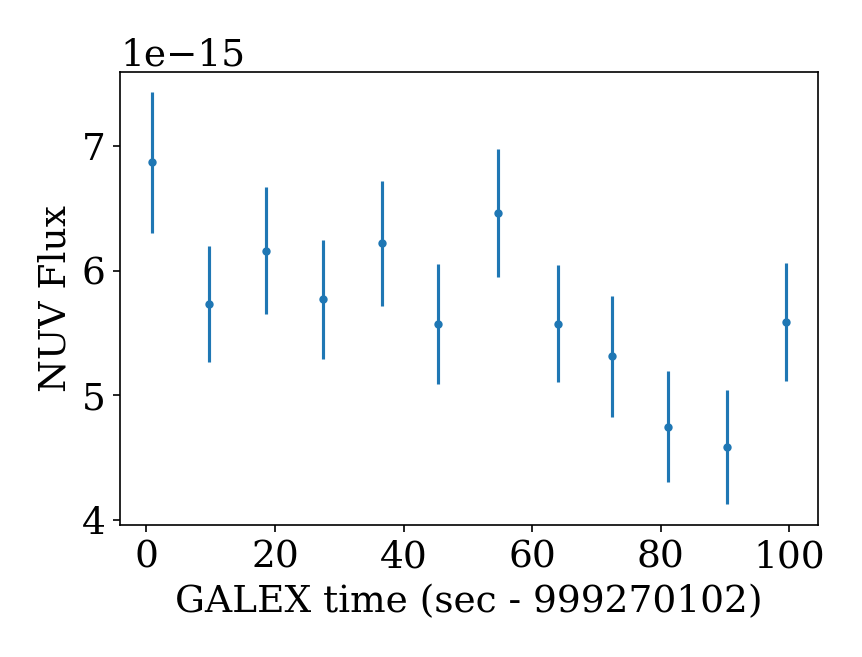
\includegraphics[width=2.7in]{KIC8462852_3_lc}
\caption{
10-second light curves from gPhoton for the 4 visits in 2012. All epochs shown (grey), and those that have no photometric warning flags set (blue), with the photometric errors for each point computed}
\label{fig:shorttime}
\end{figure}



%%%%%%%%%%%%%%%%%%%%%%
\section{Short Timescale Variability}
\label{sec:short}

gphoton gives us unique ability look for short timescale variations in the NUV.  In Figure \ref{fig:shorttime} we show the four GALEX visits covering KIC 8462852, sampled at a 10-second cadence. small variations are seen in some of the visits. we re-sampled the data at 9- and 11-sec cadence, and these are visible in each. computing a Lomb-Scargle periodogram using {\tt gatspy} \citep{gatspy} shows moderate power around 80-seconds. They appear to be primarily due to the $\sim$120 second observing cycle of the GALEX instrument in ``Petal Pattern'' mode 
A periodic signal of 0.88 days was found in \Kepler, which was presumed by \citet{boyajian2015} to be due to stellar rotation. our data are not able to verify this timescale.

nanosecond optical variability has been searched for this star \citep{abeysekara2016}, but not much else shorter than was available at 30-min cadence with \Kepler.



Since the GPhton data for this target is spread over four separate visits, we can also examine the medium-timescale variability over $\sim$70 days. In Figure \ref{fig:medtime} we show the median flux from within each of the GPhoton visits. No significant variability is seen between these visits.

%%%%%
\begin{figure}[!ht]
\centering
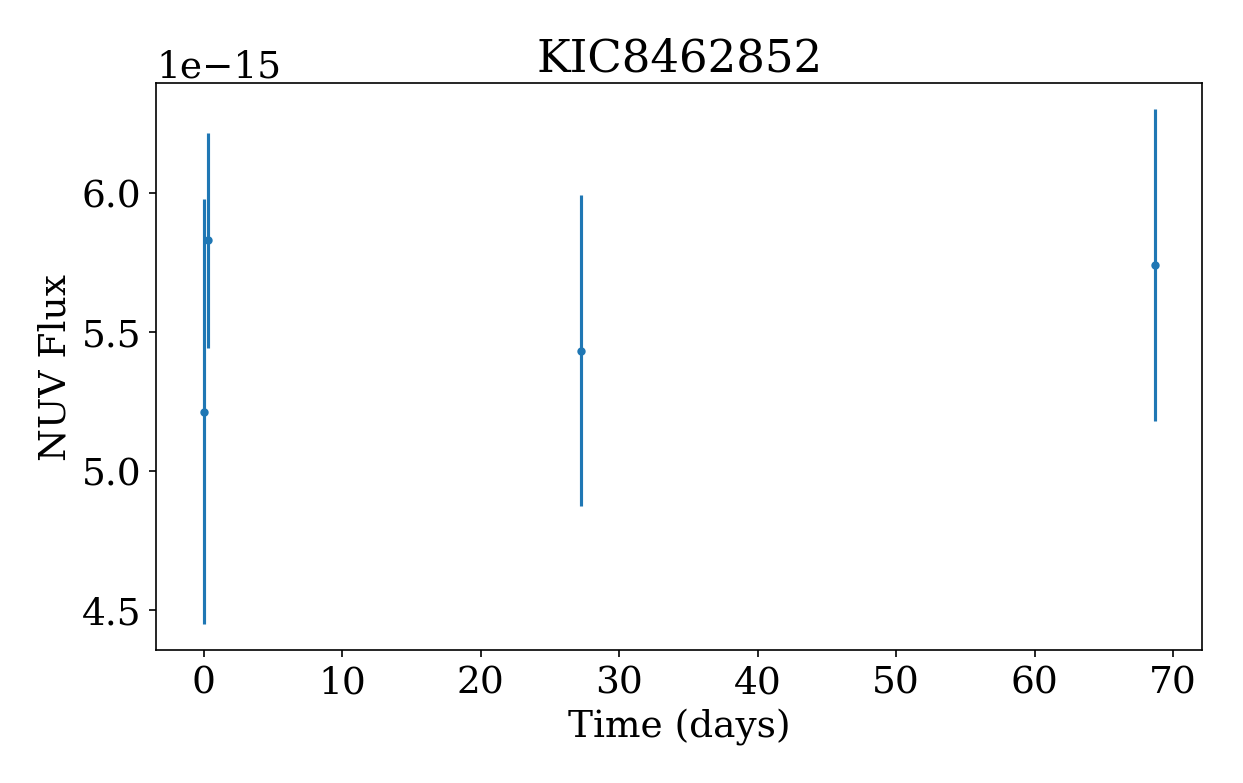
\includegraphics[width=3.5in]{KIC8462852}
\caption{median flux of the 10-sec sampled data over the $\sim$70 days of 2011 visits by GALEX. Uncertainties shown are the standard deviation in fluxes within each 10-sec sampled visit from Figure \ref{fig:shorttime}.
}
\label{fig:medtime}
\end{figure}





%%%%%%%%%%%%%%%%%%%%%%
\section{Long Timescale Variability}
\label{sec:long}

%%%%%
\begin{figure}[!ht]
\centering
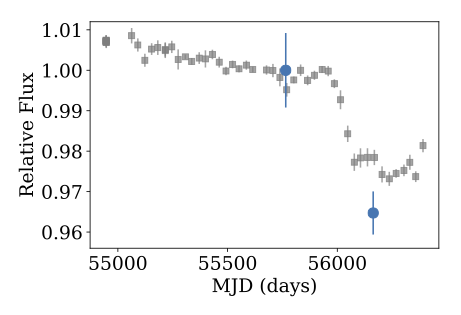
\includegraphics[width=3.5in]{KIC8462852_compare}
\caption{comparison of 2011 and 2012 fluxes (blue circles), with the \Kepler FFI data shown in \citet{montet2016} but reduced with the new ``f3'' package from \citet{montet2017} for comparison (grey squares).}
\label{fig:longtime}
\end{figure}


While the standard GALEX survey data available within GPhoton only sampled $\sim$70 days within 2011, the \Kepler field was fortunately observed again by the CAUSE/GCK survey. [INSERT DETAILS OF THIS DATA]. A catalog of the integrated fluxes and uncertainties for \Kepler targets observed in the CAUSE survey was made available by \citet{olmedo2015}


In Figure \ref{fig:longtime} we present the GALEX data for this target as observed in 2011 and 2012. The 2011 data is the final GALEX GR6 catalog flux for KIC NNNN of $16.46 \pm 0.01$ from \citet{bianchi2014}, while the 2012 data is from the GCK data of $16.499\pm0.006$ \citet{olmedo2015}. Both data were converted to fluxes and were normalized to the flux of the 2011 visit. For comparison we also show the FFI decay from \citet{montet2016}. Note: the fact that the GALEX and \Kepler FFI data are normalized to a relative flux of 1 around 2011 (MJD$\sim$55700) is a coincidence. However, the GALEX flux decays with the \Kepler FFI flux over this time baseline






%%%%%%%%%%%%%%%%%%%%%%
\section{Implications for the Nature of KIC 8462852}
\label{sec:dust}

%%%%%
\begin{figure}[!t]
\centering
\includegraphics[width=3.5in]{KIC8462852_extinction_model_1}
\caption{comparison of flux decrease observed at the effective wavelengths of the NUV and \Kepler bands (blue solid line) and a corresponding $R_V=3.1$ dust model from \citet{cardelli1989} tuned to pass through the \Kepler data (orange dashed line). The standard dust model over-predicts the NUV flux decrease given the observed \Kepler decrease from\citet{montet2016}.}
\label{fig:dust}
\end{figure}


fit with \citet{cardelli1989} dust model, using Python code from \citet{barbary2016}.



\citet{metzger2017} argued long-time fading due to stellar atmosphere recovery after a planetary in-spiral. (and possibly short-time dips due to debris) 

our added data from GALEX adds important constraint on the nature of the long timescale fading. If its dust, must have $R_V=5.0\pm0.9$ to satisfy the optical and NUV dimming. This is not typical for interstellar extinction material, though is seen for young protostars \citep[e.g.][]{hecht1982}. based on different prescriptions of the NUV extinction law, which can be very sensitive to the large ``bump'' near the GALEX NUV center wavelength.  
for example, models from \citet{fitzpatrick2009}give $R_V=5.8\pm1.6$


If the slow variability is due to dust, we can further put a weak constraint on how much dust should be present. Based on relations from \citep{guver2009}, we find that an extinction of $A_V = 0.026$ mag corresponds to 
a column density of $N_H\sim5\e{19}$ cm$^{-2}$ . Similarly, using the relations from \citet{rachford2002} that have some dependence on dust composition ($R_V$), we get an estimated $N_H\sim4.0\e{19}$ cm$^{-2}$ .




%%%%%%%%%%%%%%%%%%%%%%
\section{Summary}
\label{sec:summary}

we have provided the first independent verification of slow fading of this target

though the long timescale light curve is very sparsely sampled, the combination of NUV and optical wavelengths provides a powerful constrain on the nature of this slow dimming. 

In the hunt for other objects of this class, we are able to expand our search criteria beyond the dramatic short timescale events and slow dimming observed with \Kepler, to now include slow variability in the NUV. 



%%%%%%%%%%%%%%%%%
\acknowledgments
JRAD is supported by an NSF Astronomy and Astrophysics Postdoctoral Fellowship under award AST-1501418. 


%%%%%%%%%%%%%%%%%
\bibliography{/Users/james/Dropbox/references.bib}

\end{document}
